% !TeX encoding = UTF-8
% !TeX program = xelatex
% !TeX spellcheck = en_US

\documentclass[degree=master]{thuthesis}
  % 学位 degree:
  %   doctor | master | bachelor | postdoc
  % 学位类型 degree-type:
  %   academic(默认)| professional


% 论文基本配置,加载宏包等全局配置
% !TeX root = ./thuthesis-example.tex

% 论文基本信息配置

\thusetup{
  %******************************
  % 注意:
  %   1. 配置里面不要出现空行
  %   2. 不需要的配置信息可以删除
  %   3. 建议先阅读文档中所有关于选项的说明
  %******************************
  %
  % 输出格式
  %   选择打印版(print)或用于提交的电子版(electronic),前者会插入空白页以便直接双面打印
  %
  output = print,
  %
  % 标题
  %   可使用“\\”命令手动控制换行
  %
  title  = {工业装备状态预测\\暨模型训练加速方法研究},
  title* = {An Introduction to \LaTeX{} Thesis Template of Tsinghua
            University v\version},
  %
  % 学位
  %   1. 学术型
  %      - 中文
  %        需注明所属的学科门类,例如:
  %        哲学、经济学、法学、教育学、文学、历史学、理学、工学、农学、医学、
  %        军事学、管理学、艺术学
  %      - 英文
  %        博士:Doctor of Philosophy
  %        硕士:
  %          哲学、文学、历史学、法学、教育学、艺术学门类,公共管理学科
  %          填写“Master of Arts“,其它填写“Master of Science”
  %   2. 专业型
  %      直接填写专业学位的名称,例如:
  %      教育博士、工程硕士等
  %      Doctor of Education, Master of Engineering
  %   3. 本科生不需要填写
  %
  degree-name  = {工程硕士},
  degree-name* = {Master of Engineering},
  %
  % 培养单位
  %   填写所属院系的全名
  %
  department = {软件工程系},
  %
  % 学科
  %   1. 学术型学位
  %      获得一级学科授权的学科填写一级学科名称,其他填写二级学科名称
  %   2. 工程硕士
  %      工程领域名称
  %   3. 其他专业型学位
  %      不填写此项
  %   4. 本科生填写专业名称,第二学位论文需标注“(第二学位)”
  %
  discipline  = {软件工程},
  discipline* = {Software Engineering},
  %
  % 姓名
  %
  author  = {李思宇},
  author* = {Siyu Li},
  %
  % 指导教师
  %   中文姓名和职称之间以英文逗号“,”分开,下同
  %
  supervisor  = {邓仰东, 副教授},
  supervisor* = {Associate Professor Deng YangDong},
  %
  % 副指导教师
  %
  % associate-supervisor  = {陈文光, 教授},
  % associate-supervisor* = {Professor Chen Wenguang},
  %
  % 联合指导教师
  %
  % joint-supervisor  = {某某某, 教授},
  % joint-supervisor* = {Professor Mou Moumou},
  %
  % 日期
  %   使用 ISO 格式;默认为当前时间
  %
  % date = {2019-07-07},
  %
  % 是否在中文封面后的空白页生成书脊(默认 false)
  %
  include-spine = false,
  %
  % 密级和年限
  %   秘密, 机密, 绝密
  %
  % secret-level = {秘密},
  % secret-year  = {10},
  %
  % 博士后专有部分
  %
  % clc                = {分类号},
  % udc                = {UDC},
  % id                 = {编号},
  % discipline-level-1 = {计算机科学与技术},  % 流动站(一级学科)名称
  % discipline-level-2 = {系统结构},          % 专业(二级学科)名称
  % start-date         = {2011-07-01},        % 研究工作起始时间
}

% 载入所需的宏包

% 可以使用 nomencl 生成符号和缩略语说明
% \usepackage{nomencl}
% \makenomenclature

% 表格加脚注
\usepackage{threeparttable}

% 表格中支持跨行
\usepackage{multirow}

% 固定宽度的表格。放在 hyperref 之前的话,tabularx 里的 footnote 显示不出来。
% \usepackage{tabularx}

% 跨页表格
% \usepackage{longtable}

% 量和单位
\usepackage{siunitx}

% 定理类环境宏包
\usepackage{amsthm}
% 也可以使用 ntheorem
% \usepackage[amsmath,thmmarks,hyperref]{ntheorem}

% 参考文献使用 BibTeX + natbib 宏包
% 顺序编码制
\usepackage[sort]{natbib}
\bibliographystyle{thuthesis-numeric}

% 著者-出版年制
% \usepackage{natbib}
% \bibliographystyle{thuthesis-author-year}

% 本科生参考文献的著录格式
% \usepackage[sort]{natbib}
% \bibliographystyle{thuthesis-bachelor}

% 参考文献使用 BibLaTeX 宏包
% \usepackage[backend=biber,style=thuthesis-numeric]{biblatex}
% \usepackage[backend=biber,style=thuthesis-author-year]{biblatex}
% \usepackage[backend=biber,style=apa]{biblatex}
% \usepackage[backend=biber,style=mla-new]{biblatex}
% 声明 BibLaTeX 的数据库
% \addbibresource{ref/refs.bib}

% 定义所有的图片文件在 figures 子目录下
\graphicspath{{figures/}}

% 数学命令
\newcommand\dif{\mathop{}\!\mathrm{d}}  % 微分符号

% hyperref 宏包在最后调用
\usepackage{hyperref}




\begin{document}
\setcounter{tocdepth}{2}
\setcounter{secnumdepth}{2}
% 封面
\maketitle

% 学位论文指导小组、公开评阅人和答辩委员会名单
% !TeX root = ../thuthesis-example.tex

\begin{committee}[name={学位论文指导小组、公开评阅人和答辩委员会名单}]

  \newcolumntype{C}[1]{@{}>{\centering\arraybackslash}p{#1}}

  \section*{指导小组名单}

  \begin{center}
    \begin{tabular}{C{3cm}C{3cm}C{9cm}@{}}
      李XX & 教授     & 清华大学 \\
      王XX & 副教授   & 清华大学 \\
      张XX & 助理教授 & 清华大学 \\
    \end{tabular}
  \end{center}


  \section*{公开评阅人名单}

  \begin{center}
    \begin{tabular}{C{3cm}C{3cm}C{9cm}@{}}
      刘XX & 教授   & 清华大学                    \\
      陈XX & 副教授 & XXXX大学                    \\
      杨XX & 研究员 & 中国XXXX科学院XXXXXXX研究所 \\
    \end{tabular}
  \end{center}


  \section*{答辩委员会名单}

  \begin{center}
    \begin{tabular}{C{2.75cm}C{2.98cm}C{4.63cm}C{4.63cm}@{}}
      主席 & 赵XX                  & 教授                    & 清华大学       \\
      委员 & 刘XX                  & 教授                    & 清华大学       \\
          & \multirow{2}{*}{杨XX} & \multirow{2}{*}{研究员} & 中国XXXX科学院 \\
          &                       &                         & XXXXXXX研究所  \\
          & 黄XX                  & 教授                    & XXXX大学       \\
          & 周XX                  & 副教授                  & XXXX大学       \\
      秘书 & 吴XX                  & 助理研究员              & 清华大学       \\
    \end{tabular}
  \end{center}

\end{committee}



% 也可以导入 Word 版转的 PDF 文件
% \begin{committee}[file=figures/committee.pdf]
% \end{committee}


% 使用授权的说明
\copyrightpage
% 将签字扫描后授权文件 scan-copyright.pdf 替换原始页面
% \copyrightpage[file=scan-copyright.pdf]

\frontmatter
% !TeX root = ../thuthesis-example.tex

% 中英文摘要和关键字

\begin{abstract}
  % 论文的摘要是对论文研究内容和成果的高度概括。
  % 摘要应对论文所研究的问题及其研究目的进行描述,对研究方法和过程进行简单介绍,对研究成果和所得结论进行概括。
  % 摘要应具有独立性和自明性,其内容应包含与论文全文同等量的主要信息。
  % 使读者即使不阅读全文,通过摘要就能了解论文的总体内容和主要成果。

  % 关键词用“英文逗号”分隔,输出时会自动处理为正确的分隔符

  利用蓬勃发展的人工智能和大数据技术,
  针对工业装备特别是复杂装备实现预测式维护是工业互联网+的重要组成部分,
  能够大幅度降低装备的运行成本、全面保障装备安全稳定运行,
  对于我国制造业转型升级、跨越式发展具有极其重要的意义。
  由于工业装备数据以传感器采集的时间序列数据为主,
  因此以上问题很大程度上体现为针对时间序列的预测问题。
  
  工业装备数据来源复杂、机理多样、场景众多,
  而且数据分布上一般具有正常运行样本量巨大单故障样本稀少的特点。
  如何根据正常运行样本进行训练并同时具备故障检测能力,
  已经成为亟待解决的问题。
  
  同时, 由于其数据特点,工业人工智能摸往往存在着模型数量大、
  训练时间长、模型泛化能力差的问题,
  如何加快模型训练速度、提供模型构造效率,也成为一个迫切需要解决的问题。 

针对以上问题,本文提出了两个研究目标:

\begin{enumerate}[1)]
  \item 利用正常数据训练出满足实际应用需求、并能发现故障的时间序列预测模型;
  \item 提高时间序列模型训练效率。
\end{enumerate}
 
本文的主要贡献包括如下内容:

\begin{enumerate}
  \item 针对牵引系统设备温度监测,
  设计了基于历史信息和基于电气信号两种不同的工业装备预测模型; 
  \item 构造了基于以上模型的完整预测方案,首先应用LSTM 和 CNN 搭建时间序列预测网络,
  利用经验模态分解进行信号分解,
  对不同频率信号进行分别预测;
  并且进一步对高低频数据采用不同的采样频率;尝试应用自编码器进行相关特征处理。 
  \item 研究利用重要性采样的方法对模型训练进行加速, 设计和搭建了通用的加速框架,并且进行了实验验证,能够缩短训练过程50\%。
\end{enumerate}

  \thusetup{
    keywords = {时间序列预测, 深度神经网络, 重要性采样, 经验模态分解},
  }
\end{abstract}

\begin{abstract*}
  An abstract of a dissertation is a summary and extraction of research work and contributions.
  Included in an abstract should be description of research topic and research objective, brief introduction to methodology and research process, and summarization of conclusion and contributions of the research.
  An abstract should be characterized by independence and clarity and carry identical information with the dissertation.
  It should be such that the general idea and major contributions of the dissertation are conveyed without reading the dissertation.

  An abstract should be concise and to the point.
  It is a misunderstanding to make an abstract an outline of the dissertation and words “the first chapter”, “the second chapter” and the like should be avoided in the abstract.

  Keywords are terms used in a dissertation for indexing, reflecting core information of the dissertation.
  An abstract may contain a maximum of 5 keywords, with semi-colons used in between to separate one another.

  % Use comma as seperator when inputting
  \thusetup{
    keywords* = {keyword 1, keyword 2, keyword 3, keyword 4, keyword 5},
  }
\end{abstract*}


% 目录
\tableofcontents

% 插图和附表清单
\listoffiguresandtables  % 插图和附表清单
% \listoffigures           % 插图清单
% \listoftables            % 附表清单

% 符号对照表
% !TeX root = ../thuthesis-example.tex

\begin{denotation}[3cm]
  \item[EMD] 经验模态分解 (Empirical Mode Decomposition)
  \item[iid] 
\end{denotation}



% 也可以使用 nomencl 宏包,需要在导言区
% \usepackage{nomencl}
% \makenomenclature

% 在这里输出符号说明
% \printnomenclature[3cm]

% 在正文中的任意为都可以标题
% \nomenclature{PI}{聚酰亚胺}
% \nomenclature{MPI}{聚酰亚胺模型化合物,N-苯基邻苯酰亚胺}
% \nomenclature{PBI}{聚苯并咪唑}
% \nomenclature{MPBI}{聚苯并咪唑模型化合物,N-苯基苯并咪唑}
% \nomenclature{PY}{聚吡咙}
% \nomenclature{PMDA-BDA}{均苯四酸二酐与联苯四胺合成的聚吡咙薄膜}
% \nomenclature{MPY}{聚吡咙模型化合物}
% \nomenclature{As-PPT}{聚苯基不对称三嗪}
% \nomenclature{MAsPPT}{聚苯基不对称三嗪单模型化合物,3,5,6-三苯基-1,2,4-三嗪}
% \nomenclature{DMAsPPT}{聚苯基不对称三嗪双模型化合物(水解实验模型化合物)}
% \nomenclature{S-PPT}{聚苯基对称三嗪}
% \nomenclature{MSPPT}{聚苯基对称三嗪模型化合物,2,4,6-三苯基-1,3,5-三嗪}
% \nomenclature{PPQ}{聚苯基喹噁啉}
% \nomenclature{MPPQ}{聚苯基喹噁啉模型化合物,3,4-二苯基苯并二嗪}
% \nomenclature{HMPI}{聚酰亚胺模型化合物的质子化产物}
% \nomenclature{HMPY}{聚吡咙模型化合物的质子化产物}
% \nomenclature{HMPBI}{聚苯并咪唑模型化合物的质子化产物}
% \nomenclature{HMAsPPT}{聚苯基不对称三嗪模型化合物的质子化产物}
% \nomenclature{HMSPPT}{聚苯基对称三嗪模型化合物的质子化产物}
% \nomenclature{HMPPQ}{聚苯基喹噁啉模型化合物的质子化产物}
% \nomenclature{PDT}{热分解温度}
% \nomenclature{HPLC}{高效液相色谱 (High Performance Liquid Chromatography)}
% \nomenclature{HPCE}{高效毛细管电泳色谱 (High Performance Capillary lectrophoresis)}
% \nomenclature{LC-MS}{液相色谱-质谱联用 (Liquid chromatography-Mass Spectrum)}
% \nomenclature{TIC}{总离子浓度 (Total Ion Content)}
% \nomenclature{\textit{ab initio}}{基于第一原理的量子化学计算方法,常称从头算法}
% \nomenclature{DFT}{密度泛函理论 (Density Functional Theory)}
% \nomenclature{$E_a$}{化学反应的活化能 (Activation Energy)}
% \nomenclature{ZPE}{零点振动能 (Zero Vibration Energy)}
% \nomenclature{PES}{势能面 (Potential Energy Surface)}
% \nomenclature{TS}{过渡态 (Transition State)}
% \nomenclature{TST}{过渡态理论 (Transition State Theory)}
% \nomenclature{$\increment G^\neq$}{活化自由能(Activation Free Energy)}
% \nomenclature{$\kappa$}{传输系数 (Transmission Coefficient)}
% \nomenclature{IRC}{内禀反应坐标 (Intrinsic Reaction Coordinates)}
% \nomenclature{$\nu_i$}{虚频 (Imaginary Frequency)}
% \nomenclature{ONIOM}{分层算法 (Our own N-layered Integrated molecular Orbital and molecular Mechanics)}
% \nomenclature{SCF}{自洽场 (Self-Consistent Field)}
% \nomenclature{SCRF}{自洽反应场 (Self-Consistent Reaction Field)}



% 正文部分
\mainmatter
% !TeX root = ../thuthesis-example.tex

\chapter{引言}\label{chapter1}

\section{研究背景与意义}
据估计,在2020年,我们每个人平均每秒会产生1.7MB的数据,
仅仅在过去的两年,就产生了世界上90\%的数据,
我们每天正在产生2.5亿字节的数据\cite{siegel2013predictive}。
在快速发展的技术的推动下,我们身边产生的数据不断地增加。
随着工业4.0时代的到来,由于现代生活各个方面的数字化,
例如,物联网(Internet of Things, IoT)技术正在不断深化发展,
时间序列数据的数据量急剧增加。

大量数据的增加,“大数据”时代的到来,带来了很多新的机遇,
也给研究人员带来了新的挑战。
我们现在在处理、存储和分析大数据的能力方面也取得了很多进展,
例如在计算集群上用分布式的方式处理和存储数据方面,及用人工智能
(AI, Artificial intelligence)和机器学习
(ML, Machine learning)的方式处理大量非结构化
数据内容的能力等,这些方面都有了很大的发展等。

现代装备的复杂性和高度集成性也导致了故障表现形式的复杂化,
而且由于设备装态受环境和工况影响比较大,
传统的基于机理的分析方式没有办法涵盖所有的故障问题。
工业大数据是智能制造和制造服务化的重要组成部分,
在制造、电力、航空、轨道交通、船舶、石油等各方面都有很多具体的应用。
工业装备状态预测,尤其是复杂装备的状态预测,
是装备状态监测及运维服务系统的基础。
基于数据的自动化的解决方案,
能够大大地降低装备的运行成本,保障装备运行的稳定性和安全性,
对制造业的跨越式的发展有着极其重要的意义。

时间序列是按照时间顺序对特定过程进行观测而形成的数值序列。
时间序列分析的目的在于通过挖掘反映数据变化规律的模式,
在理解时间序列的基础上实现分类和预测,从而支持针对相应
自然和社会现象的决策。
高效能时间序列分析在金融、生物信息、自然灾害预测、
过程控制等方面具有极其重要的作用。

针对历史IoT数据进行预测具有十分重要的意义。
一方面可以通过数据预测未来趋势,从而进行优化决策,例如针对风力发电的风力预测;
另一方面,时间序列预测也可以用于实时故障检测,
由于工业数据往往存在故障样本稀少的问题,
可以通过建立基于正常数据的预测模型,
然后通过分析预测模型(反映正常运行模式)和实际数据的残差进行故障预测。
通过数据驱动的方式重建机理,将预测式分析手段应用于装备部件、系统甚至是整车
级别的故障预测、推理和剩余寿命估计,能全面地提高设备的健康管理水平,
大大地提高运维效率,和装备的出勤率,节约运维和设备运行的成本和效率。

\section{问题描述与主要挑战}
  \subsection{问题描述及研究目标}
  \paragraph{问题描述}~{}

    本课题针对工业装备状态这一类时间序列的预测问题,研究如何训练高准确度的模型,及训练过程的加速问题。
  \paragraph{研究目标}~{}\label{goal}

    时间序列的预测问题的典型解决方法是应用传统的概率统计模型,
    由于其准确率高、模型相对简单、鲁棒性好等优点,应用广泛。
    但是传统方法特征提取自动化程度低、验证依靠经验和人工分析。
    面对海量数据,深度学习具有自动化特征提取、对机理和人工依赖程度较低的优点,
    成为未来的发展趋势。
    因此,本文采用基于深度学习的时间序列预测框架。

    然而,现有的深度学习方法的有以下三个问题:
    \begin{enumerate}
      \item 难以跟踪快速跳变数值。深度神经网络在回归问题上往往难以适应快速变化的数据,导致平均精度高、但是极值点附近误差较大的问题,然而极值点附近又往往是预测的重点。
      \item 模型训练速度慢。在用深度学习处理时间序列问题中,模型优化的计算量大,需要的样本数量多,训练速度慢。导致在很多场景下,深度学习在时间序列上的应用相较于传统方法,并没有明显的优势。
      \item 模型定制要求高。和深度学习应用到图像分类问题中不同,
      时间序列问题中数据之间的分布并没有显著的相似性。
      如果训练一个全局的深度学习模型,在具体的某一时间序列数据上,
      模型的效果可能会特别差\cite{lebedev2018speeding}。时间序列问题的模型迁移能力差,
      无法将神经网络应用于各类不同的任务。工业数据情况复杂多变,
      往往需要针对问题定制模型,甚至每台机器都需要单独的模型。
    \end{enumerate}

    深度神经网络的训练时间很长,加之需要多个不同的模型。
    训练速度极大地限制了深度学习在时间序列问题上的发展。
    针对以上提出的现有的深度学习方法存在的问题,
    本课题提出了两个的研究目标:
    \begin{enumerate}
      \item 训练出准确度能满足实际应用需求的时间序列预测模型。
      \item 快速而且有效地训练时间序列模型。
    \end{enumerate}


  \subsection{时间序列预测的挑战性}
    自然和社会现象的错综复杂决定了时间序列的复杂性,
    本课题针对的工业装备IoT数据更具有以下鲜明特点:
    \begin{enumerate}[(1)]
      \item 动态性:工业数据往往具有时变和非稳态的特点,
      即数据背后的统计分布和规律随时间变化,
      同时各种突发事件、偶然因素的影响也会造成非趋势性和非周期性的不规则变动。
      \item 多样性:需要多种模型。
      时间序列问题的数据之间的分布并没有显著的相似性。
      如果训练一个全局的模型,在具体的某一时间序列数据上,
      模型的效果可能会特别差。时间序列问题的模型迁移能力差,
      无法将神经网络应用于各类不同的任务。
      工业数据情况复杂多变,往往需要针对问题定制模型,
      甚至每台机器都需要单独的模型。
      \item 小样本:工业装备IoT数据的典型特点是故障类型呈长尾分布,
      正常运行样本极为丰富,特点故障样本稀少。
      样本的严重不均衡导致故障和非故障的分类十分困难,
      传统的监督式分类方法在这种情况下并不适用。
      \item 高维度:一方面,随着各方面硬件技术的不断发展,
      实际应用中数据的采样频率不断提高,因此时间序列的长度也不断变大,
      仅仅把时间序列看作单纯的一维向量数据来处理不可避免地会带来维数灾难等问题;
      另一方面,很多实际应用中的时间序列数据往往包含多个变量(multivariate),
      这些变量之间往往存在复杂依赖关系。
    \end{enumerate}

\section{研究内容与主要贡献}
以电网数据和告诉机车数据为研究对象,针对时间序列回归预测问题,
研究高准确度预测模型以及加速训练技术和方法。
针对章节\ref{goal}中提出的两个研究目标,研究内容分为以下几个部分。
\begin{enumerate}[(1)]
  \item 针对时间序列预测问题,调研和应用了深度神经网络模型结构和方法。
  \item 设计合理的模型训练框架,对时间序列模型的训练进行了加速。
  \item 对具体的电网问题和轨道车辆走行部问题,对数据进行了分析和处理,搭建了时间序列模型训练和预测的系统。
\end{enumerate}

针对具体的研究内容,设计的研究方案包括如下主要内容:

\begin{enumerate}
  \item 设计了基于历史信息和基于电气信号两种不同的工业装备预测方案。
  \item 应用LSTM和CNN搭建时间序列预测网络,并在此基础上对预测系统进行改进。
  利用经验模态分解进行信号分解,对不同频率信号进行分别预测;并且进一步对高低频数据采用不同的采样频率;
  尝试应用自编码器进行相关特征处理。
  \item 应用重要性采样的方法对模型训练进行加速。
  \item 设计和搭建了通用的加速框架,并实验其效果,验证其稳定性。
\end{enumerate}

\section{组织结构}
本文总共分为六个章节。

第 \ref{chapter1} 个章节引言中,对问题本身进行了阐述,包括研究背景与意义,和问题描述与挑战分析。

第 \ref{chapter2} 个章节国内外研究现状,主要是对预备知识的阐述和研究现状的调研与分析。

第 \ref{chapter3} 、 \ref{chapter4} 、 \ref{chapter5} 是文章的主要工作内容的介绍。
这三个章节中,第 \ref{chapter4} 、 \ref{chapter5} 章介绍了本文的两大块的主要内容,
分别是工业装备的预测,和利用重要性采样对训练过程进行加速。
在第 \ref{chapter3} 中则对这两部分内容中实验的设定和数据部分进行了说明,
数据部分包含数据说明、数据特点分析和数据预处理几大部分。

在最后第  \ref{chapter6} 章中,对全文的研究做了总结,并提出了未来的展望。
% !TeX root = ../thuthesis-example.tex

\chapter{国内外研究现状}\label{chapter2}
\section{引言}
本章节对研究内容相关的文献进行了调研,对研究现状进行了阐述、分析和总结。
同时为了方便理解研究内容、方便阅读,也对涉及到的一些相关的背景知识进行了介绍。
\section{时间序列预测方法}
  针对章节\ref{goal}中提出的第一个研究目标:训练出准确度能满足实际应用需求的时间序列预测模型。
  这里调研了常用的时间序列预测的模型和方法,和一些提高预测效果的手段,
  同时也对不同模型的特点进行了分析。
\subsection{时间序列预测常用模型}

  处理时间序列的常用方法包括两类,
  一类是传统的统计模型例如ETS和ARIMA,第二类是基于深度神经网络。

  基于深度神经网络的模型预测方法近年来越来越具有竞争力。
  传统的统计学模型依然具有其兼顾准确率高、模型相对简单、鲁棒性好、高效等优势。
  然而,更复杂,更高维度和以及包含噪声的现实世界中的时间序列数据
  无法用带有参数的解析方程来描述,因为动力学太复杂且未知,
  传统浅层方法因为只包含一个小的非线性操作的数量,
  没有能力准确地模拟这种复杂的数据。
  从未标记数据中学习特征的优点是可以利用丰富的未标记数据,
  并且可以学习比手工制作的特征更好的特征。
  这两个优点都减少了对数据专业知识的需求。

  近年来,在时间序列预测领域,也有关于标准框架的基础工作支持深度学习在时间序列预测问题上的发展。
  出现了为时间序列预测研究设计的
  GluonTS开源框架\cite{DBLP:journals/corr/abs-1906-05264}。

  \begin{figure}
    \centering
    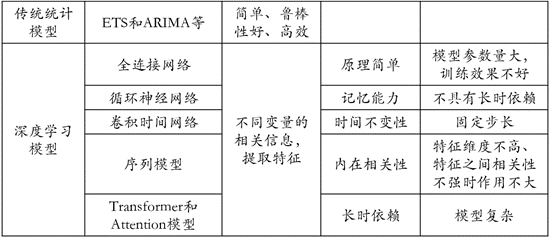
\includegraphics[width=\linewidth]{figures/预测典型模型.png}
    \caption{应用于时间序列预测的典型模型类型及其特点总结}
    \label{tab:prediction models}
  \end{figure}
  常用的深度神经网络包括循环神经网络(如LSTM和GRU)、
  序列模型、卷积神经网络、Transformer和Attention模型。
  M4竞赛结果表明\cite{MAKRIDAKIS202054},
  准确率最好的模型都结合了传统统计模型和深度学习模型,
  或多种深度学习模型。在时间序列预测问题上,
  没有哪一种绝对优势的模型,各种模型都有其结构上的优势特点。
  不同模型的优势特点如表\ref{tab:prediction models}。

  \paragraph{循环神经网络在时间序列预测问题上的应用效果及问题}~{}

    DeepAR提出基于LSTM的时间序列概率自回归预测模型
    \cite{salinas2020deepar},
    用LSTM模型建模未来时间步中的贝叶斯模型。
    近年提出的模型中,结合了指数平滑方法的混合RNN模型\cite{smyl2020hybrid}
    在M4预测竞赛中成为最终的优胜模型\cite{MAKRIDAKIS202054}。
    循环神经网络由于其独特的记忆机制\cite{hewamalage2021recurrent},
    一直都是处理时间序列问题的最通用选择之一,
    常用的模型结构如长短时记忆LSTM和门控循环单元GRU。

    GRU-ODE-Bayes网络\cite{de2019gru}构建了一个连续版本的门控循环神经网络,
    利用贝叶斯的方法更新,在多项任务中取得了很好的效果。

    但是循环神经网络也有其缺点,比如对并行训练的支持不好、
    不能捕捉过长的时序依赖关系等。
    所以人们也一直没有放弃对其他网络结构在时间序列预测问题上的探索。

  \paragraph{序列模型能有效捕捉相关性及构造时变模型}~{}

    常见的序列模型一般包括编码器和解码器两部分。
    能够捕捉时间序列数据之间的相关性。
    目前效果较好的序列模型是由多个RNN组成。

    \begin{figure}
      \centering
      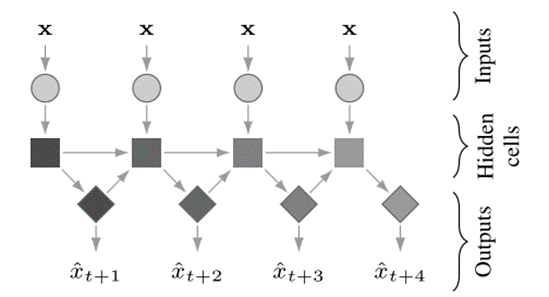
\includegraphics[width=0.8\linewidth]{figures/ForecastsNet 网络结构.png}
      \caption{ForecastsNet 网络结构}
      \label{tab:ForecastsNet}
    \end{figure}

    ForecastNet\cite{dabrowski2020forecastnet}中采用Dense连接的方式,
    如图\ref{tab:ForecastsNet}所示,
    实现了时变的模型结构,同时通过交错输出的方式,
    有效地缓解了梯度消失的问题,
    在多步的时间序列预测问题上得到了不错的准确度。  
  
  \paragraph{应用于时间序列预测的卷积神经网络}~{}
  
    \begin{figure}
      \centering
      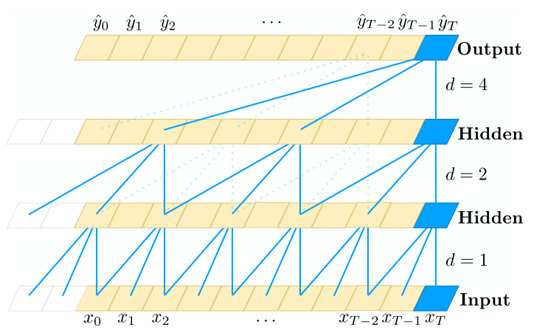
\includegraphics[width=0.8\linewidth]{figures/TCN空洞卷积结构.png}
      \caption{TCN空洞卷积结构}
      \label{tab:TCN}
    \end{figure}
    早在上个世纪80年代末,卷积的结构就被应用于序列问题上
    \cite{lecun1989backpropagation}。
    卷积神经网络通过卷积和参数共享来实现位移不变性的效果\cite{amari2003handbook},
    能够应用在时间序列模型上,具有时间不变性的特性。
    在建模序列数据问题上,通过多个评价系统\cite{chung2014empirical}的测试,
    达到了相当不错的效果,
    明显优于循环神经网络\cite{binkowski2018autoregressive}。
    卷积神经网络相比循环神经网络,
    结构上支持并行,计算速度方面能够得到有效地保证。
    也有相关工作\cite{shi2015convolutional}结合了卷积神经网络和循环神经网络,
    用卷积层替换了长短时记忆网络中原有的全连接层。

    以Temporal Convolution Networks (TCN) 为代表的更先进的卷积神经网络,
    结合了更大的卷积范围和残差跳跃连接,在序列建模任务的训练上,
    取得了很好的效果\cite{bai2018empirical,pascanu2013construct}。
    TCN应用了空洞卷积的卷积结构,
    如图 2中的感受野足够大,能够捕捉序列中的长时依赖信息,
    而且利用了残差连接,有效地提升了模型的准确率。
  
\subsection{提高预测效果方法}
  \paragraph{经验模态分解}~{}

    经验模态分解(Empirical Mode Decomposition, EMD)
    方法被认为是自2000年来,以傅立叶变换为基础的线性和稳态频谱分析的一个重大突破。
    
    对于非线性数据尤其是非平稳数据,直接处理会非常难,
    但是这类数据就比较适合用经验模态分解来处理,
    经验模态分解在这类数据的处理上会具有明显的优势。
    
    经验模态分解也常常会被用在信噪比低的数据上提升数据的信噪比。
\section{对时间序列模型的训练加速}
  \subsection{模型训练加速方法研究现状}
  时间序列模型的训练速度严重制约了深度学习在时间序列上的应用。
  模型的训练加速一般有特征、样本、模型几个方向的思路。对特征进行降维、筛选有效样本、
  利用多级模型在保证准确率的情况下降低使用的模型的复杂度。

  另外图像领域对训练加速的研究对时间序列模型也有一定的借鉴意义。
  为了保证阐述的完整性,这里列出了其他的一些可以参考的图像问题加速的方法。
  以常用的卷积神经网络为例,常用的加速方法包括:
  (1)张量分解,(2)低精度的运算和其他量化方法,(3)对大网络进行剪枝,
  (4)用Teacher-Student方法通过训练小网络得到大网络,
  (5)设计高效的网络结构,用启发式的方法找到最精简的网络结构,
  (6)网络结构的自动搜索等\cite{lebedev2018speeding}。
  近年来,研究者们将模型训练的效果提升和过程加速的注意力转移到重要性采样上来。

  \subsection{筛选有效样本(重要性采样)}
  重要性采样(Importance Sampling)是统计学中估计某一分布性质时使用的一种方法。
  该方法从与原分布不同的另一个分布中采样,而对原先分布的性质进行估计。

  重要性采样被应用于提升凸优化问题的随机优化方法的收敛速度上,
  例如构造核分类器\cite{bordes2005fast}、
  用随机过程优化正则化损失\cite{zhao2015stochastic}等。
  另外一方面,在深度神经网络领域,
  样本筛选的方法也被应用于解决困难样本的处理问题,
  例如在嵌入学习问题中\cite{wu2017sampling},也被应用于解决样本不平衡的问题。

  深度神经网络花费了很多重复的计算量在处理很容易拟合的样本上,
  这些样本在训练一段时间后,就能被忽略掉,并不会影响最终的模型效果,
  在训练过程的某些时间开始忽略这样的样本,能大大地节省模型优化的计算量。
  也就是说,在训练过程中,不同的样本对收敛过程起到的作用效果是不一样的,
  很多样本在很少的几个轮次之后就能被很好地分类或者拟合,通过对样本的筛选,
  能够在较少影响准确率的情况下有效地加速训练过程。

  近年来的一些工作表明\cite{needell2014stochastic},
  重要性采样的方法的加速原理是降低随机梯度下降过程中梯度估计的方差,
  最优的采样分布应该和样本的梯度范数成正比。
  所以重要性采样一般围绕梯度范数展开,但是由于梯度范数的计算复杂度过高,
  另外一种常用的思路是通过训练过程的损失来对梯度范数进行拟合,
  从而计算样本重要性。
  通过损失来计算样本重要性的方法通常有很多超参数需要调优,
  并且对梯度范数拟合得不够。
  为了探索一种更好的训练数据选择策略,
  包括课程学习(curriculum)和自步学习(Self-paced Learning)
  在内的先前工作都采用了简单的启发式规则,例如打乱序列长度来训练语言模型,
  或放弃损失值大于手动定义的阈值的训练样本。
  这种人为定义的规则在一定程度上受限于某些任务,
  不能推广到更广泛的学习场景,
  因为不同的学习任务可能会产生不同的最佳数据选择规则,
  甚至一个学习任务可能也需要具有各种属性的数据才能在不同的训练阶段进行优化。

  Yang Fang等人应用强化学习的方法来选取样本\cite{fan2016neural}。
  通过强化学习来设计一个训练数据的过滤器(Neural Data Filter, NDF)插入到网络输入层之前,
  在训练的过程中动态筛除一部分对训练益处不大的数据,从而减少训练数据量。
  该方法有两个直观的原则:一方面,数据选择策略应该是通用的,
  这样就可以自然地将其应用于不同的学习场景,
  而无需进一步的人工设计。 另一方面,该策略应具有前瞻性,
  因为它在训练的每个步骤中的选择都会带来更好的长期回报,
  而不是暂时适应当前阶段。

  NDF的基本工作流程是:给定当前训练中的网络的状态和当前mini-batch数据的状态(states)   ,
  输出一组动作(action) ,  是一个0,1向量,
  它的维度和mini-batch的大小相同,
  每个元素代表了mini-batch中对应的数据是否应该被剔除。
  利用强化学习的方法来建立过滤器的过程包括以下几个步骤,首先通过现有的采样的policy,
  输入当前的模型状态和待采样样本状态,输出采样的结果,然后将样本输入模型中,
  得到实际的梯度下降的效果的Reward,继而用Reward对采样的policy进行优化。

  \subsection{重要性采样介绍}

  \paragraph{蒙特卡洛积分}~{}

  提到重要性采样首先要介绍蒙特卡洛积分的概念。

  蒙特卡洛是一类算法的总称,是用随机抽样和统计模拟的方法,来进行数值计算。
  它的基本做法是,做大量重复实验来统计频率,
  根据伯努利大数定律,当样本数足够多时,频率会无限接近于概率,
  所以理所当然,可以通过频率来估计概率。

  对于求解积分$\int_a^b f(x)dx$,经典的方法是我们需要找出$f(x)$的原函数$F(x)$。
  但是,在求积分的过程中,积分的原函数在很多情况下都不是很容易获得,那么我们就无法应用经典的求解积分的方法。

  蒙特卡洛积分是蒙特卡洛算法的具体应用。
  蒙特卡洛方法在估计$\int_a^b f(x)dx$积分时,将其表示为一个均匀随机变量的期望,如下,
  \begin{equation}
      \theta=\int_a^b f(x)dx = (b-a)\int_a^b f(x) \frac{1}{b-a}dx=(b-a)E(f(X)), X\sim U(a,b)
  \end{equation}
  其中$U(a,b)$代表在[a,b]之间的均匀分布。从而可以通过如下算法来得到积分估计的结果:
  \begin{enumerate}
      \item 从分布$U(a,b)$中产生i.i.d样本$x_1,x_2,x_3,...,x_n$;
      \item 计算$f(X)$期望的估计值$\overline{f(X)}=\frac{1}{n}\sum_{i=1}^{n} f(x_i)$;
      \item 得到$\hat{\theta}=(b-a)\overline{f(X)}$。
  \end{enumerate}
  容易得到,估计值$\hat{\theta}$的期望和方差分别为,

  $E\hat{\theta}=\theta$,
  $Var(\hat{\theta})=(b-a)^2 Var(\overline{f(X)})=\frac{(b-a)^2}{n}Var(f(X))$

  但是基于均匀分布的估计方法,不能应用于无穷积分的估计,
  而且当被积函数在积分区间上的分布不是很均匀时,抽样的效率会比较低。

  \paragraph{重要性采样}~{}

  前面的蒙特卡洛积分经典计算方法采用均匀分布作为加权函数,会有抽样效率的问题,
  重要性采样就是一种利用合理的加权函数,提高抽样样本效率的计算方法。
  和经典的计算方法相比,重要性采样的加权函数不再是均匀分布。
  设随机变量$X$的概率密度函数是$g(x)$。记$Y=\frac{f(x)}{g(x)}$
  \begin{equation}
      \theta=\int_a^b f(x)dx = \int_a^b \frac{f(x)}{g(x)}g(x)dx=EY
  \end{equation}
  再通过简单的蒙特卡洛积分方法估计$EY$:
  \begin{equation}
      \hat{\theta}'=\hat{EY}=\frac{1}{n}\sum_{i=1}^{n}y_i=\frac{1}{n}\sum_{i=1}^{n}\frac{f(x_i)}{g(x_i)}
  \end{equation}
  此处$x_1,x_2,x_3,...,x_n$为从g(x)中抽取的样本。
  用这个方法估计的参数的方差为
  $Var(\hat{\theta}')=Var(Y)/n$。当$Y$为常数时方差为0。
  所以,$f(x)$的选择目标应该是尽量接近$g(x)$。

  % \subsection{优化理论} % Todo
% !TeX root = ../thuthesis-example.tex


\chapter{时间序列数据分析与处理}\label{chapter3}


\section{引言}
  在本章节中,对实验的情况进行了具体的说明,
  交待了实验环境,实验参数等。

  同时对数据相关的问题进行了阐述。
  对实验中用到的数据进行了说明,
  同时说明了数据预处理的流程和具体的方法,
  以及采用相关方法的动机、实际效果等。


\section{数据及评价指标说明}
  本文中应用的数据主要包括电网数据和列车走行部数据,都是实时采集的实际场景中的工业装备状态数据。
  下面对这两种数据的具体情况分别进行了说明。

  % !!!说明数据分别应用到了哪些地方
  \subsubsection{电网数据说明}
    本文实验中采用的电网数据,是基于青岛永磁实验台,
    按线路条件(包括牵引、匀速、制动),跑典型工况,采集的相关数据。

    数据在150t、192t、222t三种不同载荷下分别采集,
    在为10Hz、100Hz、100kHz三种不同采集频率的下,采集到不同特征列数据。

    在表\ref{tab:features2}中对各特征列进行了详细的说明。
    \begin{table}
        \centering
        \caption{电网温度预测模型中用到的主要特征说明}
        \begin{tabular}{lclclclcl}
          \toprule
          特征    & 通道名称 &采集频率&采集方式 &特征说明                                       \\
          \midrule
          电机温度   & AI\_Motor2Temp1\_gui &10Hz &PTU采集 & 待预测特征之一\\
          PU温度   & AI\_PUTemp\_gui &10Hz &PTU采集 & 待预测特征之一\\
          网流   & AI\_BusNegCurrent\_gui &10Hz &PTU采集 & 输入特征之一\\
          U相电流瞬时值   & AI\_PhaseUCurrent2\_gui &10Hz &PTU采集 & 输入特征之一\\
          U相电流有效值   & AI\_PhaseUCurrent2\_RMS\_gui &10Hz &PTU采集 & 输入特征之一\\
          W相电流瞬时值   & AI\_PhaseWCurrent2\_gui &10Hz &PTU采集 & 输入特征之一\\
          W相电流有效值   & AI\_PhaseWCurrent2\_RMS\_gui &10Hz &PTU采集 & 输入特征之一\\
          环境温度   & PT2\_ &100Hz &数采系统 & 输入特征之一\\
          电机速度   & Mot2\_speed\_rpm\_gui &10Hz &PTU采集 & 输入特征之一\\
          
          \bottomrule
        \end{tabular}
        \label{tab:features2}
      \end{table}
    !!!补充完整
  \subsubsection{列车走行部数据说明}
    本文实验采用的数据包含列车底盘(又名走行部)的监测数据,
    包含各轴承温度、驾驶档位、输出功率、环境温度、当前轨道的地理位置情况等相关数据。

    需要通过预测轴承温度的方式来判断轴承的运行状态。

    本文中实验用的是车号为5103的列车的数据,在表\ref{tab:features1}中对各特征列进行了详细的说明。
    在清洗完成后,还剩88401条可用数据,跨时234天,平均时间间隔为228.6秒,
    但是采样间隔分布比较不均匀,例如列车停运时采样间隔会比较长。

    \begin{table}
      \centering
      \caption{列车轴温预测模型中用到的主要特征说明}
      \begin{tabular}{ll}
        \toprule
        特征       & 特征说明                                       \\
        \midrule
        采集时间      & 用于数据分段和序列处理 \\
        车号          &\\
        1~6个轴的测试温度 & 待预测特征。共6个轴,每个轴六个测试点。 \\
        环境温度1、2  & 两个点采集到的环境温度,用于预测轴温的特征 \\
        主发电机温度  & 用于预测轴温的特征\\
        风机1、2温度  & 用于预测轴温的特征\\
        

        \bottomrule
      \end{tabular}
      \label{tab:features1}
    \end{table}
  \subsubsection{评价指标}
    均方误差(MSE,Mean squared error)是比较常用的反映估计量和被估计量之间差异程度的一种度量。
  
    但是均方误差作为评价指标也有它存在的问题。比较大的一个问题就是对异常值比较敏感,
    如果样本中有个别异常值出现,会对均方误差的影响比较大,导致评估的结果并不鲁棒。
  
    针对这个问题,在数据预处理的数据清洗阶段做出了一些处理,去掉了一些明显的异常点。
    % \subsection{数据集和实验基准说明}

\section{数据特点分析}
  \subsection{工业装备状态数据特点}
  工业装备数据一般采集于实际的工业装备系统,由于系统本身十分复杂,
  机理很难分析,很难对其进行建模分析。
  而且由于数据本身会存在噪声干扰,特性也比较复杂,
  通过传统的时间序列的分析方法也很难对其进行建模和抽取特征。
  
  \subsubsection{电网数据特点}
    \begin{enumerate}
      \item 电网数据来源于几种不同的采集方法,不同采集方法的采样频率会有差异。
      \item 如电压电流这类特征会有很明显的周期性。
    \end{enumerate}
  \subsubsection{列车轴温数据特点}
    \begin{enumerate}
      \item 数据波动十分剧烈。这份数据采集所在的区域所在的环境温度波动剧烈,
      如图\ref{fig:environment temperature change}所示,
      昼夜温差很大,低温低于15摄氏度,高温高于42摄氏度。
      
      \item 虽然在数据表中包含了地理位置信息,
      但是当前轨道的地理情况(坡度、弯度等)很难精确捕捉。
      \item 根据采集时间来看,列车的运行并不是一个连续的过程,
      会存在停运的情况,而且数据采集的过程也不连续。所以不能直接作为一个长时间序列来进行处理,
      需要对数据进行分段。
    \end{enumerate}
    \begin{figure}
      \centering
      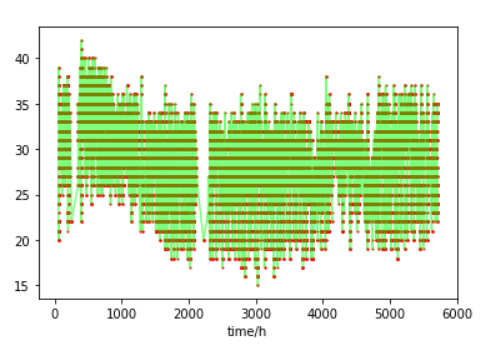
\includegraphics[width=0.8\linewidth]{figures/5303evn_tpt.png}
      \caption{5103号列车数据中环境温度变化图(横轴是时间,纵轴是环境温度,单位为摄氏度)}
      \label{fig:environment temperature change}
    \end{figure}

  \subsection{时间序列数据平稳性分析}
    \paragraph{平稳性分析的意义}~{}

    平稳性分析能够确定模型是否具有统计分析的意义。
    虽然利用深度学习建模并不是基于统计来对数据进行处理,
    但是平稳性分析能够检测序列是否具备被预测的基础,例如白噪声就不能被预测。

    这一个步骤主要是为了对待预测的数据的性质和预测难度有一个了解,方便后续选择合适的预测方法。
    
    % \paragraph{平稳性分析的具体方法和结论}~{} %Todo

\section{数据预处理}
数据的预处理包括如下的几个主要部分:数据读入、数据清洗、数据重采样、数据分段、数据标准化、
经验模态分解、数据窗口处理、划分训练集和测试集这些部分。下面会对这些内容分别进行阐述。
视数据特点的不同,个别的流程可能可以省略。
  \begin{figure}
    \centering
    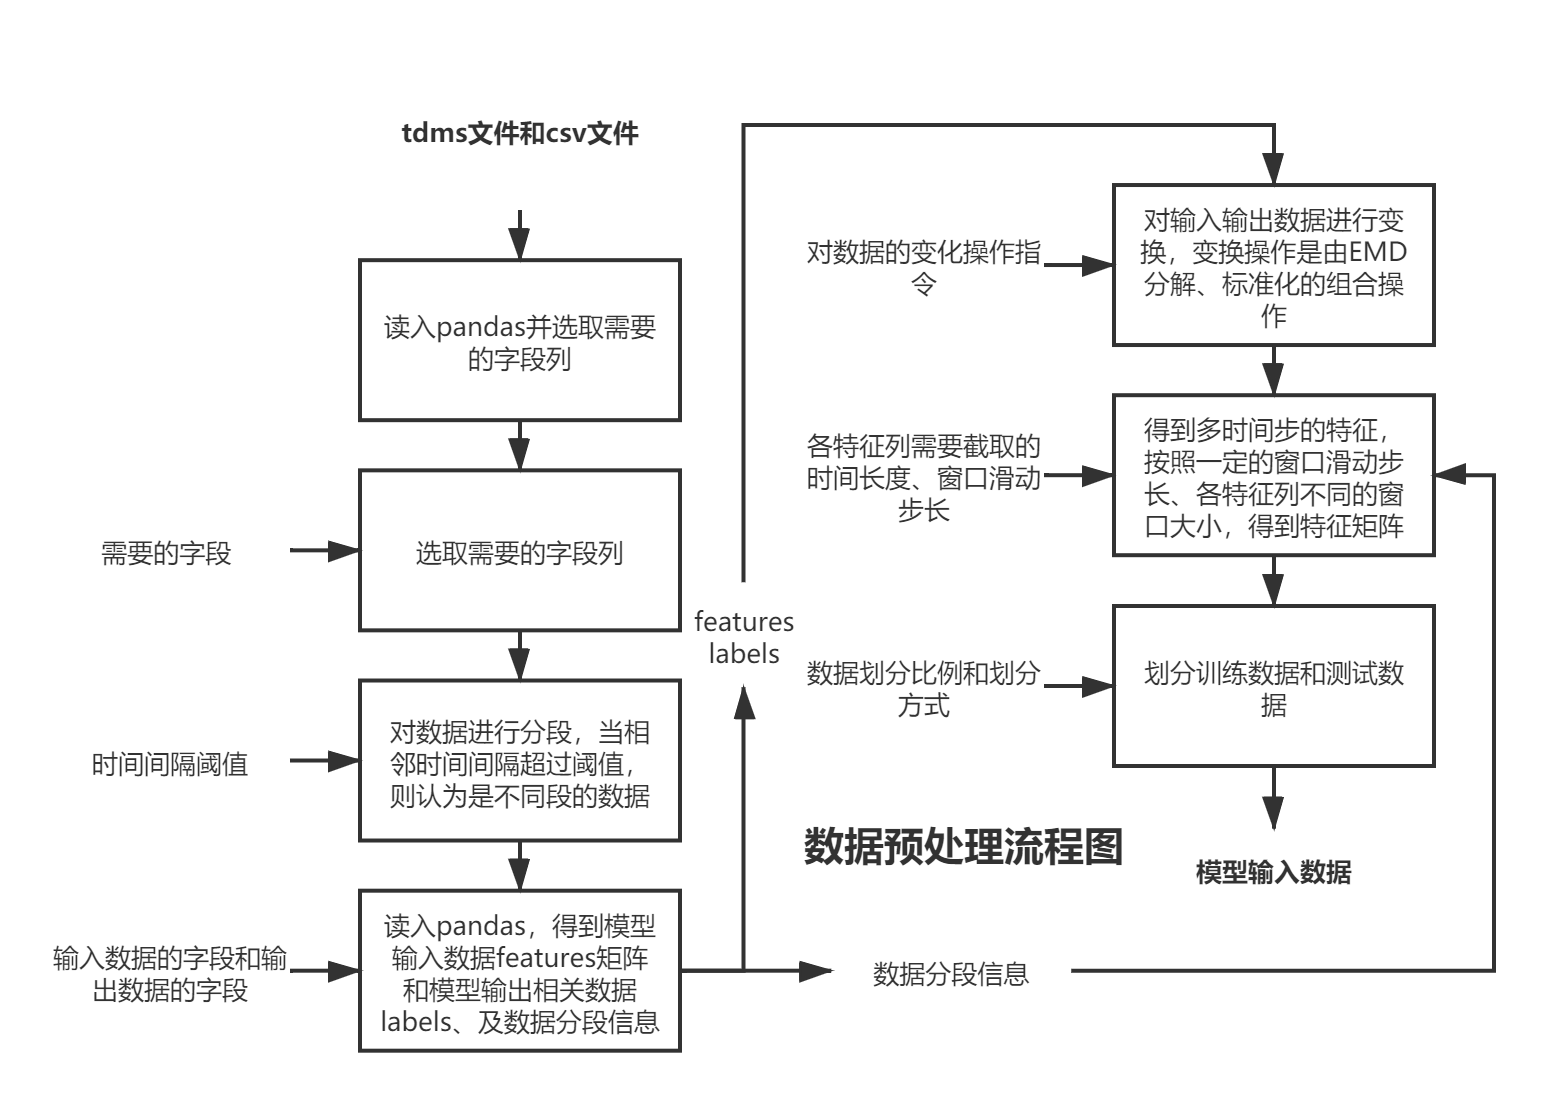
\includegraphics[width=1.1\linewidth]{figures/数据预处理流程.png}
    \caption{电网数据分段及划分处理流程图}
    \label{fig:data preprocess}
  \end{figure}
  \subsection{数据导入及清洗}
    电网原始数据存储在tdms文件和csv文件中,把数据读入pandas之后进行处理。
    列车轴温原始数据存储于dmp文件中,需要通过oracle数据库工具进行导入。

    在列车轴温数据中,导入后的数据存在问题。首先是存在着部分列的数据格式问题,
    打印出来发现是因为个别数据显示为“异常温度”或者是“-”。另外会有些数据的时间
    标记是默认的最小值的数据。
    用简单的处理数据缺失的方法来处理,由于数据量可观,可以直接在数据表
    中删除异常的样本点。

  \subsection{数据重采样}
  \begin{figure}
    \centering
    
    \begin{subfigure}[b]{0.45\textwidth}
        \centering
        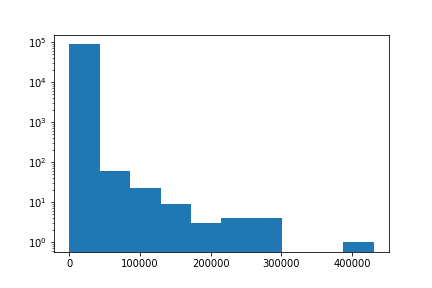
\includegraphics[width=\textwidth]{figures/time_intervals_distribution_log.png}
        \caption{采样间隔分布(log)}
        \label{fig:time_interval_log}
    \end{subfigure}
    \hfill
    \begin{subfigure}[b]{0.45\textwidth}
      \centering
      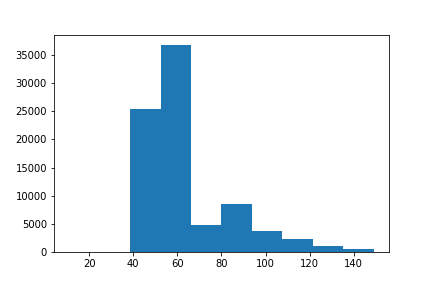
\includegraphics[width=\textwidth]{figures/time_intervals_distribution150.png}
      \caption{小于150秒的采样间隔分布}
      \label{fig:time_interval}
    \end{subfigure}
    
    \caption{列车走行部数据采样时间间隔分布直方图(横坐标:间隔(s),纵坐标:频次)}
    \label{fig:time intervals}
  \end{figure}
  需要注意的是,这一步对电网数据和列车轴温数据需要进行的操作是不一样的。
  
  在电网数据中,数据本身有固定的采样频率,采样间隔都是统一的,
  只是不同特征的采样频率不一样。

  但是在列车走行部数据中,如图\ref{fig:time intervals}中给出的采样时间间隔分布所示,
  采样点并不均匀的,就必须进行均匀间隔的重采样。

  \subsection{数据分段}
  首先介绍为什么需要对数据进行分段,在列车走行部数据中,如图\ref{fig:time intervals}中给出的采样时间间隔分布所示,
  采样点是十分不均匀的,间隔可能长达40000秒(约1天左右),也可能很短,50秒左右。
  如果只是进行简单的重采样,如果重采样的采样间隔过短,那在原始数据采样间隔很长的地方,
  会造成大量的数据冗余,对模型的训练也并没有好处;如果重采样的采样间隔过长,又会导致
  信息的过度丢失。

  所以这里提出一个数据分段的解决方案,通过设定一个合理的时间间隔阈值,如果两个点之间的
  时间间隔过长,我们则认为它们属于两个不同的数据段。

  关于时间间隔阈值的选择问题。可以将所有数据的时间间隔分布用直方图统计出来,
  再根据统计出来的结果选择出一条比较明显的分界线。

  为了找到重采样的合理阈值,这里对采样间隔进行了如\ref{fig:time intervals}直方图分析,
  大部分的采样间隔都集中在150秒以下,通过如\ref{fig:time_interval}
  中对150秒以下的间隔的进一步分析可以得到,70秒是一个比较合理的阈值。

  \subsection{整理数据表并通过滑动窗口取模型输入}
  在清洗完数据并对数据分好段之后,把需要用到的数据整理成一张二维的数据表。
  每一列是一个属性,每一行是一个采样点的数据。
  !!!滑动窗口示意图

  % \paragraph{输入输出的格式定义}~{} %Todo

  % 为了灵活方便,将输入输出定义为如下的字典格式:
  % \begin{minted}{Python}
  %     {(start_1, end_1) : [feature_1_1, feature_1_2, ...],
  %     (start_2, end_2) : [feature_2_1, feature_2_2, ...], ...}
  % \end{minted}

  % 其中start和end是相对时间而不是绝对时间。注意在input和output中相对时间的参考点需要一致。

  % 例如下面的定义方式,
  % \begin{minted}{Python}
  % input_attrs = {(-history_length, predicted_length) : features,
  %               (-history_length, 0) : labels} # 输入
  % output_attrs = {(0, predicted_length) : labels} # 输出
  % \end{minted}
  % 代表!!!


  \subsection{数据标准化}
  \begin{figure}
    \centering
    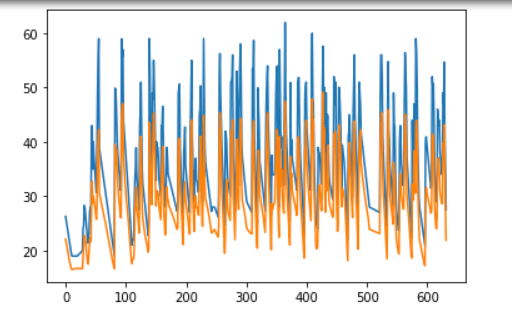
\includegraphics[width=0.8\textwidth]{figures/normalization.png}
    \caption{数据标准化前预测效果示意图}
    \label{fig:before normalization all points}
  \end{figure}
  数据预处理过程需要对数据进行标准化。如果没有标准化,会出现的问题是,
  预测趋势还是对的,但是对高温和低温的极值附近的预测很差,Accuracy结果比较好但是MSE差,
  这也是由于MSE的结果会比较受个别值的影响。
  如图\ref{fig:before normalization all points}所示。


  \begin{figure}
    \centering
    
\includegraphics[width=\textwidth]{figures/标准化流程.png}
    \caption{数据标准化流程}
    \label{fig:pipeline of normalization}
  \end{figure}
  
  采用的标准化的方式是普遍被应用的控制均值和控制标准差的方式。
  具体的公式如\ref{eq:normalizaiton}所示,
  数据标准化的处理流程如\ref{fig:pipeline of normalization}所示,
  需要将预测结果反标准化之后再进行应用和计算评价标准的值。

  \begin{equation}\label{eq:normalizaiton}
    z=(x-u)/s
  \end{equation}

  其中,$u$是x的平均值,$s$是x的标准差。

  \begin{figure}
    \centering
    
    \begin{subfigure}[b]{0.45\textwidth}
        \centering
        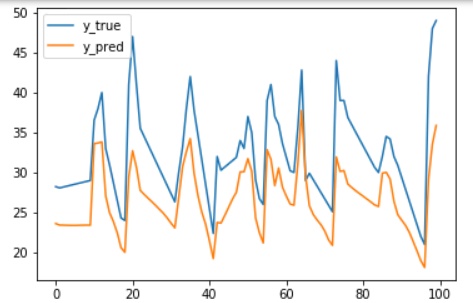
\includegraphics[width=\textwidth]{figures/normalization1.png}
        \caption{数据标准化前}
        \label{fig:before normalization}
    \end{subfigure}
    \hfill
    \begin{subfigure}[b]{0.45\textwidth}
      \centering
      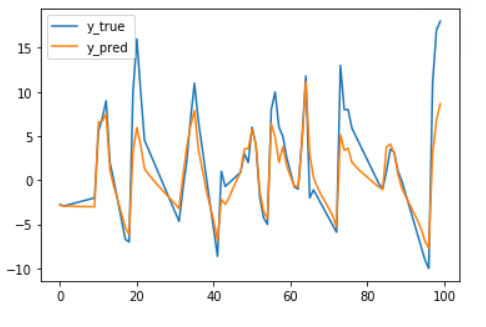
\includegraphics[width=\textwidth]{figures/normalization2.png}
      \caption{数据标准化后}
      \label{fig:after normalization}
    \end{subfigure}
    
    \caption{数据标准化效果说明图}
    \label{fig:normalization}
  \end{figure}

  为了更清晰的对比,在\ref{fig:normalization}中,截取了预测结果的片段进行对比。
  标准化前预测效果如\ref{fig:before normalization}所示。
  在加入标准化处理后,预测效果有了明显地改善。
  标准化后预测效果如\ref{fig:after normalization}所示。

  \subsection{不同序列划分方式}\label{subsection_diffrent_divide}
    训练集和测试集有如下两种不同的划分方式:
    \begin{enumerate}
      \item 第一种是序列化的顺序划分方式。
      以 7:3 的划分比例为例,即按照时间顺序,前 70\% 的数据作为训练集,后 30\% 的数据作为测试集。
      \item 第二钟是随机划分的方式。同样以 7:3 的划分比例为例,
      随机取70\%的样本点作为训练集,剩下30\%的样本点作为测试集。
    \end{enumerate}

    \begin{figure}
      \centering
      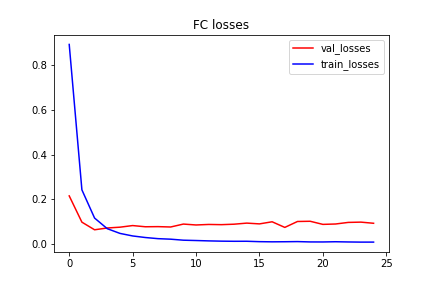
\includegraphics[width=0.5\textwidth]{20210327_1505/FC losses.png}
      \caption{出现过拟合问题的网络训练过程loss变化}
      \label{fig:overfit FC}
    \end{figure}
    
    \paragraph{序列化的划分方式下的过拟合问题}~{}

    不同的序列划分方式会导致实验结果有很大的差别。
    在序列化的划分时,很容易出现在训练集上效果很好,在测试集上效果不好的情况。
    图\ref{fig:overfit FC}是在序列化的样本划分方式下,
    应用全连接网络,训练得到的训练和验证集上的loss变化情况。
    如图\ref{fig:overfit FC},很明显训练出现了过拟合问题。
    分析原因是因为序列化的划分方式中的训练集和测试集,
    会由于工况的区别,有着很大的差异,给模型效果带来了挑战。

    但是在随机化的划分方式中则不容易出现这种问题。这也很容易理解,
    这和训练集和测试集的样本分布的相似度有关,随机划分的训练集和测试集的样本基本同分布。

    \paragraph{采样两种划分方式实验的原因}~{}

    这里之所以采用了两种划分方式进行实验,也是因为这两种划分方式各有其特点和不可替代的实际意义。
    序列化的划分方式更加接近实际中使用的场景,我们的模型在实际使用中,不可能将未来的数据拿来训练。
    但是由于资源的限制,实验用到的数据有限,而研究对象的情况会比较复杂,
    所以实际情况中会使用更多数据来训练模型,理论上当数据足够多时,会涵盖更多的数据情况,
    模型的应用效果也会更加接近随机划分训练集和测试集。

    实际的情况下模型的应用效果可能介于两种划分方式之间,所以这里对两种数据划分方式都展开了研究。
\section{实验环境}
  \begin{table}
      \centering
      \caption{实验环境}
      \begin{tabular}{ll}
        \toprule
        环境        & 版本                                        \\
        \midrule
        操作系统        & Ubuntu 18.04.3 LTS                          \\
        \bottomrule
      \end{tabular}
      \label{tab:env}
  \end{table}

  \begin{table}
    \centering
    \caption{软件环境}
    \begin{tabular}{lll}
      \toprule
      软件环境名称        & 安装包版本信息          & 安装来源                              \\
      \midrule
      Cuda        & V10.0.130     & 官网 \\
      Python      & 3.8           & Conda                              \\
      Tensorflow  & 2.4.1             & pip                          \\
      Pandas        &  1.2.2    & pip  \\
      Numpy        &    1.19.5   & pip \\
      Sklearn         &   0.24.1  & pip   \\
      EMD-signal     &  0.2.13 & pip \\

      \bottomrule
    \end{tabular}
    \label{tab:software}
  \end{table}
  本文的实验都是在Linux系统下搭建完成,语言是Python,利用GPU进行模型的训练与测试。

  深度学习框架方面,本文的实验都基于Tensorflow 版本2.4.1进行,
  应用了Tensorflow2最新的Keras接口。
  具体的实验环境和安装包配置如表\ref{tab:env}和表\ref{tab:software}所示。
  \subsection{实验说明}
    需要注意的是,为了消除随机因素的影响,
    如果没有特别说明,那文中给出的实验结果都是基于三次重复实验的平均结果。
    \subsection{选用Tensorflow2编写的优势}
    首先对比下动态图和静态图的特点。旧版本的Tensorflow一直采用的是静态图的机制,
    而被学术界研究人员广泛应用的Pytorch是基于动态图的机制。
    静态图是指,在图被构建之后,在模型运行之时,计算过程中,图是无法修改的。
    动态图反之,在计算过程中可以对图进行修改。
    由于静态图计算过程中图无法修改,所以可以在运行前进行一些优化例如融合部分Operation。
    但是也会因为图融合等原因,静态图在调试方面具有较大的难度,无法提供断点和单步调试功能,
    而且也会非常的不直观。
  
    Tensorflow不仅在部署上相对于其他框架有着独特的优势,而且Operation全面,生态良好。
    在升级Eager模式后,能够兼顾静态图运行效率快,和动态图代码简洁方便调试的优点。
  

\section{本章小结}



% !TeX root = ../thuthesis-example.tex


\chapter{工业装备状态预测}\label{chapter4}
\section{引言}
本章节介绍了工业装备状态预测的相关内容,包括整体方案的设计,和应用的具体方法,
详细地说明了设计的动机、和实际的效果。

工业装备状态预测的一个重要的应用就是将其应用到预测式故障检测中。

故障检测的一个很直接的思路是,将问题定义成一个分类问题,
分类结果分别是正常和存在故障两种状态,
这样也能通过历史数据训练神经网络模型,得到我们想要的结果。
但是在工业装备状态预测下,
作为分类问题建模存在的问题是样本极度地不平衡。
设备发生故障的情况相对正常情况会很少,
甚至是从来没有出现过故障。
在这样的情况下,分类的难度会特别大。

\begin{figure}
    \centering
    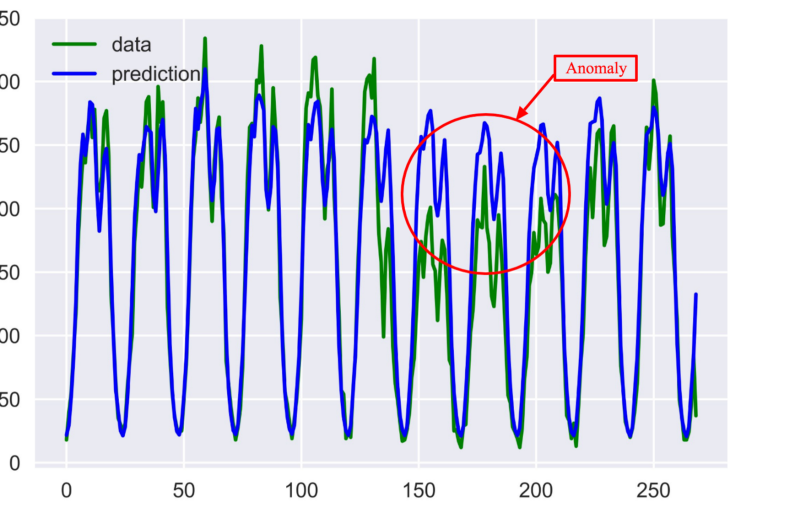
\includegraphics[width=0.6\linewidth]{figures/预测式故障检测}
    \caption{预测式故障检测示意图}
    \label{fig:prediction-fault-detection}
\end{figure}

如图\ref{fig:prediction-fault-detection}中所示,
当实际采集到的工业装备状态数据和预测数据发生较大的偏差时(图中红圈部分),
我们就可以认为是装备发生了故障。
这个前提是需要被检测到的故障会引起相应检测状态的变化,
例如在很多装备或者电子元器件中,
如果发生温度偏离正常运行状态过高,就可以认为是发生了故障。

\begin{figure}
  \centering
  
\includegraphics[width=0.8\linewidth]{figures/列车轴温预测系统流程框架图.png}
  \caption{列车轴温预测系统流程框架图}
  \label{fig:prediction_system}
\end{figure}

以列车走行部作为状态预测为例,
可以设计如图\ref{fig:prediction_system}的故障预测系统。
分为数据整理、数据预处理与分析、模型预测、应用到实际系统调试几个模块。

为了能达到能够上车调试的效果,需要对模型进行不断地迭代和优化,
直到预测的效果能够达到某一个特定的阈值。
这部分我们只关注预测的结果,可以和上车调试部分独立出来,成为一个单独的模块。
在下面的部分,我们只讨论工业装备状态预测的部分,
主要关注如何提升预测的效果,减小预测结果和实际结果之间的偏差。

\section{工业装备状态预测方案}
\subsection{系统设计}

  \begin{figure}
    \centering
    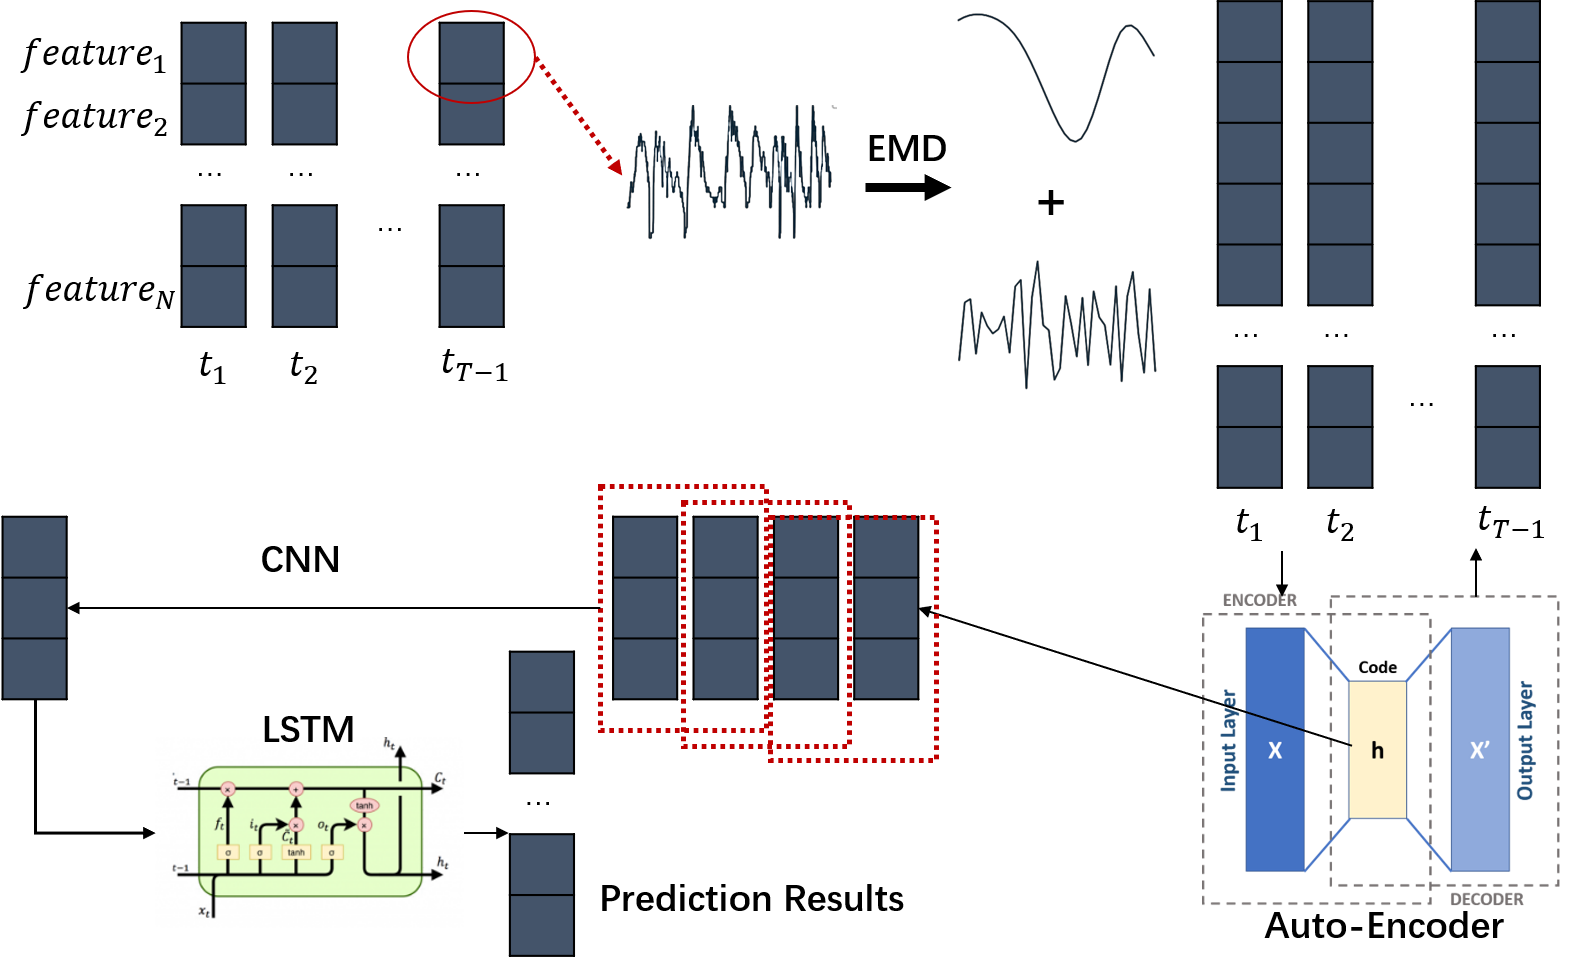
\includegraphics[width=\linewidth]{figures/prediction_system.png}
    \caption{工业装备状态预测部分系统设计}
    \label{fig:prediction system}
  \end{figure}

  如\ref{fig:prediction system}图中所示,这里给出了整体预测方案的系统设计方案。
  \begin{enumerate}
    \item 针对极值部分数据突变的预测技术。
    由于极值部分变化剧烈,往往预测效果不好。
    解决这个问题的一个方案就是对信号进行频率分解,
    这样输入的特征中会包含不同频率的信号特征,能够更好地预测极值部分的数据值。
    所以应用经验模态分解对时间序列进行信号处理,提取出不同频率的信号分量。
    \item 针对序列难建模的特点,提出应用CNN+LSTM组合的模型结构。
    \item 针对工业序列噪声大、特征之间相关程度高的特点,利用Auto-Encoder部分进行特征相关性的提取。
  \end{enumerate}
  

\subsection{方法说明}
在这一个小的章节中,将会对工业装备状态预测方案中采取的具体方法进行分别的说明。
\subsubsection{经验模态分解信号处理}
  \begin{figure}
    \centering
    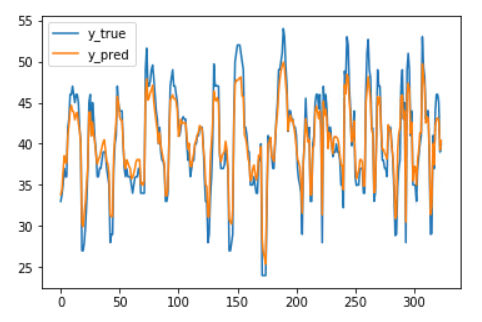
\includegraphics[width=0.8\linewidth]{figures/EMD动机.png}
    \caption{模型在高频处会预测效果差示意图}
    \label{fig:EMD motivation}
  \end{figure}
  通过实验观察发现,如图\ref{fig:EMD motivation}中所示的模型预测结果示意图
  (其中y\_true是真实值,y\_pred是预测值),
  模型预测结果的低频分量效果较好,
  但是容易在尖峰等轴温快速变化的位置预测效果相对较差。
  于是想通过EMD分解,可以提取不同频率的信号特征,进而提升模型预测效果。
  % Todo: EMD效果
\subsubsection{对高低频数据不同采样频率}
  为了进一步优化模型,在简单EMD方法的基础上,又进行了一些改进。
  由于EMD方法会将数据分解成多个不同的频率的数据,
  对于低频数据,采样太过密集会导致数据过于冗余,
  而对于高频数据,采样过于稀疏会导致高频部分数据失真。
  所以很容易想到,我们可以对不同频率的数据在输入模型前进行不同的采样频率的处理,
  在减少特征维度的同时,尽可能地提升数据的质量和模型预测效果。

\subsubsection{使用Layer Normalizaiton}
需要注意的是,由于后续需要利用重要性采样进行训练加速,为了统一,
模型中统一使用Layer Normalizaiton取代Batch Normalization。
这是因为,在重要性采样中会根据样本的重要性进行采样,
那么一个batch的样本不再是从原分布中随机产生,
不再满足和同分布的特点,那么Batch Normalization对于不同的batch的效果将不会是一致的。
会导致训练出现问题。

\subsubsection{不同时间序列预测的模型方案对比}
本文对比了几种不同模型在实验数据上的预测效果,下面分别介绍这几种模型的结构。

本文被用来对比的实验基准网络是一个全连接网络,

本文实现了长短时记忆网络,

通过实验测试了这几种不同网络的实际效果,
\subsubsection{自编码器在特征提取上的应用}
以上考虑了多个时间步上特征提取的模型结构问题,
但是在单个时间步上的多个特征之间,可能存在很强的相关性,
而特征的相互关系并不能用以上的模型结构表述,需要进一步处理。
这里提出利用Auto-Encoder结构捕捉特征之间的相关性。

需要注意的是,Auto-Encoder不需要完整地嵌入网络中,
只用将Encoder部分加入预测网络中,将Encoder的输出值输入其余部分的网络。
而且,这部分的网络无需参与后续的整个网络的梯度更新过程,只需要单独进行训练。

应用自编码器主要有两方面的目的,一方面自编码器自带的结构特征可以用来进行特征提取和降维,
另外一方面,自编码器具有降噪的效果,工业装备状态数据是实际采集到的数据,难免会存在很多噪声,
通过自编码器的应用,能够有效地减少噪声对模型的干扰。

那这里为什么选择用自编码器来进行降维,和常用的降维方法例如PCA
(Principal component analysis,主成分分析)方法对比。
PCA 方法只适用于线性降维,其他的降维方法也会受到数据的局限性,
但是自编码器降维的好处是利用深度神经网络来进行建模,对数据的拟合能力很强。
但是,自编码器降维在数据量比较小的时候容易出现过拟合的问题,
所以相对于PCA 方法而言,自动编码器更适用于复杂的大型数据集。
本论文讨论的主要针对工业装备状态这种长时间数据,采集到的数据很多,所以不用担心过拟合的问题。
% \paragraph{自编码器相关性处理}~{}
\paragraph{自编码器效果}~{}

通过实验我们发现,不是所有的工业装备状态预测的数据都适合用自编码器在特征维度进行降维。
例如在火车走行部的轴温预测中,各个不同的轴的温度会同步变换,
之间有比较强的相关性,而且这种相关性独立地存在于当前各个轴的温度状态中,
不需要额外的历史信息,解码器就能恢复出数据。

所以判断是否能够应用自编码器进行特征提取,我们可以通过训练的自编码器的输入和输出的比较,
如果差别比较小,说明编码器部分的信息损失比较小。

当然当出现自编码器效果不好时,也可以通过尝试别的不同结构的自编码器进行处理,
例如这里可以尝试编码器和解码器都是更加适用于序列处理的网络结构,例如LSTM模块,
但是在这里不作过多展开和研究。
\subsubsection{防止过拟合的策略}
针对在\ref{subsection_diffrent_divide}中提出的,
在序列化的划分方式下出现的过拟合问题,采用了加dropout的方式进行解决。
在后面应用LSTM时,也采用了同样的加dropout方式,同样也不存在过拟合问题。

\subsection{两种不同的状态预测方法}
对于状态预测有两种方式,一种是通过历史数据回归,
另外一种是结合历史数据和当前的其他可获得的电气信号预测。
这两种预测方式都有其各自的特点和适用的应用场景。

第一种通过历史数据回归的状态预测方法,它的应用场景更为广泛,
第二种需要获得当前的其他电气信号,有的场景下受到传感器数据收集速度或者数据传输速度的限制,
即时的信号并不那么容易获取,第一种方法就不会有这样的限制。

但是第一种方法也会存在相应的问题,有的时候会发生工况等状态的变化,
这样情况下简单通过历史的信息回归信息是不完备的。

\section{实验结果}

\subsection{往前预测多步结果}

  \begin{figure}
    \centering
    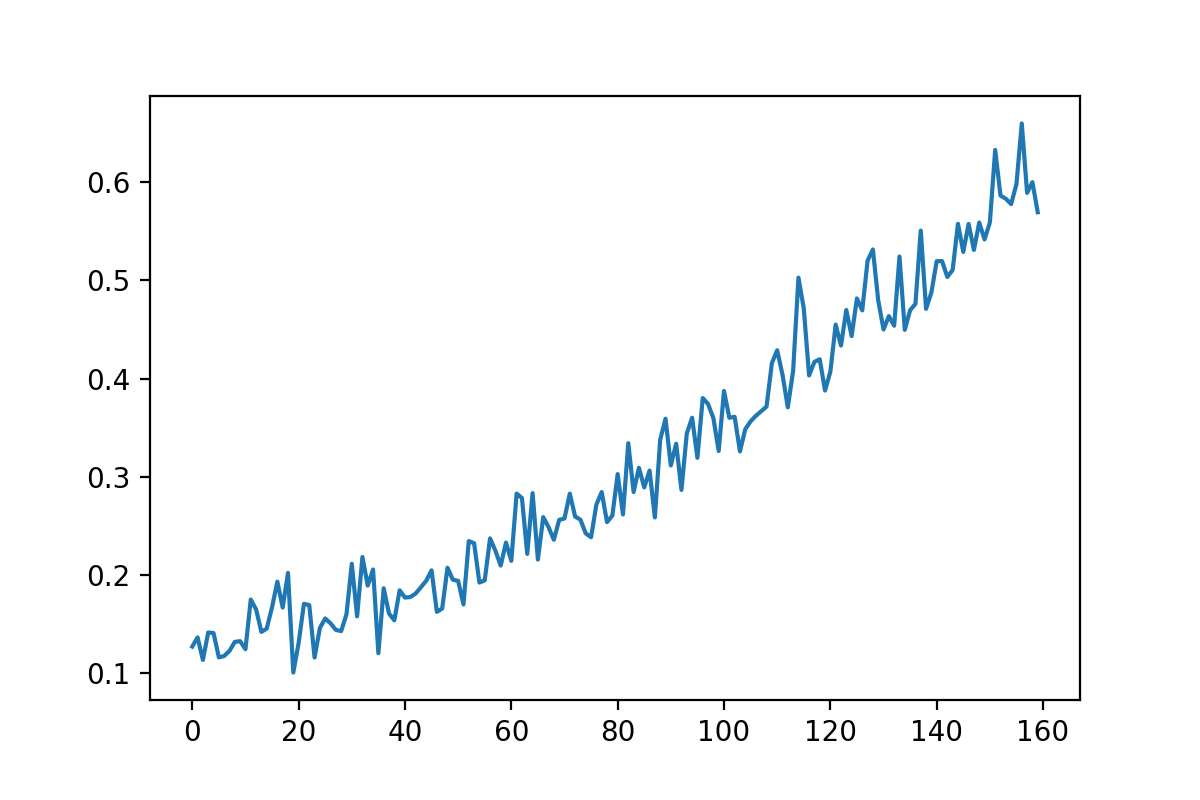
\includegraphics[width=0.8\linewidth]{figures/往前预测多步均方误差.png}
    \caption{往前预测多步均方误差(横轴坐标值代表往前预测的步数,纵轴是均方误差)}
    \label{fig:multi-step}
  \end{figure}

  预测的效果和设定的往前预测的时间长度相关。
  自回归往前预测第i步(i取1-160)的均方误差如图\ref{fig:multi-step}中所示,
  可以看到,往前预测得越远,均方误差越大,预测效果越差。
\subsection{防止过拟合的策略实验结果}

  \begin{figure}
    \centering
    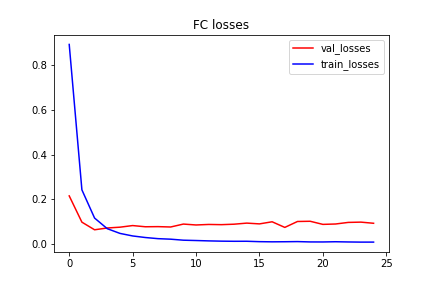
\includegraphics[width=0.5\textwidth]{20210327_1505/FC losses.png}
    \caption{出现过拟合问题的网络训练过程loss变化}
    \label{fig:overfit FC 1}
  \end{figure}

  \begin{figure}
    \centering
    \begin{subfigure}[b]{0.45\textwidth}
      \centering
      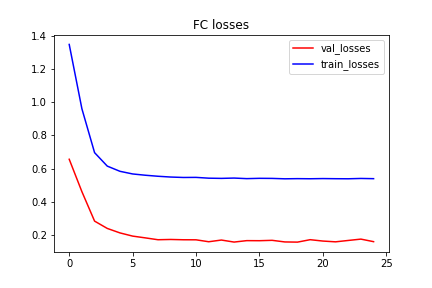
\includegraphics[width=\textwidth]{20210327_2017/FC losses.png}
      \caption{FC losses with dropout}
      \label{fig:FC losses with dropout}
    \end{subfigure}
    \hfill
    \begin{subfigure}[b]{0.45\textwidth}
        \centering
        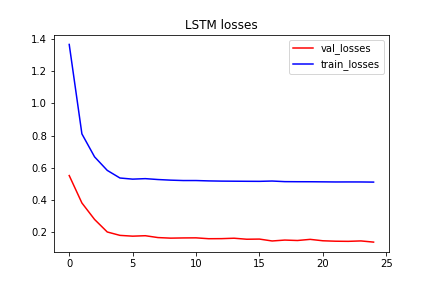
\includegraphics[width=\textwidth]{20210327_2017/LSTM losses.png}
        \caption{LSTM losses with dropout}
        \label{fig:LSTM losses with dropout}
    \end{subfigure}
       \caption{过拟合策略效果图:加了dropout之后的模型loss曲线变化}
       \label{fig:losses with dropout}
  \end{figure}

  如图\ref{fig:FC losses with dropout}中所示,
  对比前面图\ref{fig:overfit FC 1}中的结果,
  不再出现训练一段时间后训练集loss虽然一直在下降,但是验证集的loss反而再上升,
  而且训练集的效果远远好于测试集效果这样的情况。
  在模型过拟合方面有了明显改进。
  说明加dropout模块的方法十分有效。

\subsection{两种不同方法的工业装备状态预测的结果}
  
  \begin{table}
    \centering
    \caption{基于历史数据,150、192、222三组不同载荷下,电机温度预测均方误差结果}
    \begin{tabular}{lclcl}
      \toprule
      载荷       & 训练集MSE & 测试集MSE                                   \\
      \midrule
      150    & 0.357 & 0.334                                \\
      192 & 0.328 & 0.358                                     \\
      222 & 0.197 & 0.190                  \\
      \bottomrule
    \end{tabular}
    \label{tab:regression motor results}
  \end{table}

  \begin{table}
    \centering
    \caption{基于历史数据,150、192、222三组不同载荷下,PU温度预测均方误差结果}
    \begin{tabular}{lclcl}
      \toprule
      载荷       & 训练集MSE & 测试集MSE                                    \\
      \midrule
      150    & 0.011 & 0.017                                \\
      192 & 0.020 & 0.022                                     \\
      222 & 0.038 & 0.037                 \\
      \bottomrule
    \end{tabular}
    \label{tab:regression PU results}
  \end{table}
  
  \begin{table}
    \centering
    \caption{基于电气信号,150、192、222三组不同载荷下,电机温度预测均方误差结果}
    \begin{tabular}{lclcl}
      \toprule
      载荷       & 训练集MSE & 测试集MSE                                   \\
      \midrule
      150    & 0.014 & 0.670                                \\
      192 & 0.004 & 0.034                                    \\
      222 & 0.042 & 1.925                 \\
      \bottomrule
    \end{tabular}
    \label{tab:prediction motor results}
  \end{table}

  \begin{table}
    \centering
    \caption{基于电气信号,150、192、222三组不同载荷下,PU温度预测均方误差结果}
    \begin{tabular}{lclcl}
      \toprule
      载荷       & 训练集MSE & 测试集MSE                                    \\
      \midrule
      150    & 0.001 & 0.031                                \\
      192 & 0.004 & 0.032                                     \\
      222 & 0.026 & 0.610              \\
      \bottomrule
    \end{tabular}
    \label{tab:prediction PU results}
  \end{table}
  
  下面对两种不同方法分别进行实验,每种方法分别应用到电机温度预测和PU温度预测两个场景下,
  给出了在三种不同载荷情况下,训练集的MSE和测试集的MSE的最终结果。

  
  \ref{tab:regression motor results}和\ref{tab:regression PU results}
  给出的是第一种方法--基于历史信息的预测方法的结果,
  \ref{tab:prediction motor results}和\ref{tab:prediction PU results}
  给出的是第二种方法--基于电气信号的预测方法的结果。

  通过上面的结果可以看到,基于电气信号的方法的训练集MSE明显更小,而且差别比较悬殊,差了10倍以上,
  说明这样的方法的确提供的信息更完备。

  但是测试集的效果却反而不是很好,在基于电气信号的方法中,
  虽然数据提供的信息量更多,但是模型效果反而更差。
  分析原因是因为过拟合导致的,数据中的噪声也会导致这样的问题,加上MSE的数值本身就容易受到个别异常点的影响,
  所以导致了测试集MSE的结果比较差。



\section{本章小结}
在本章中讨论了关于工业装备状态预测的相关问题,
主要目标是搭建一个预测效果好的深度神经网络模型,
对不同的模型结构进行了研究和对比,同时提出了一些提高模型预测效果的方案。

% !TeX root = ../thuthesis-example.tex


\chapter{实验说明}

\section{引言}
\section{实验设置}
\subsection{深度学习框架}
\subsection{实验环境}

\section{基于时间序列预测的故障检测系统}
\subsection{系统概述}
\subsection{数据说明}
\subsection{方法定义}
\subsection{模型的训练与应用}

\section{不同训练加速方法的对比实验}
\subsection{评价指标}
\subsection{数据集和实验基准说明}
\subsection{模型训练}
\subsection{对比实验}
\subsection{分析实验}

\section{本章小结}



% % !TeX root = ../thuthesis-example.tex

\chapter{总结与展望}


\section{本文总结}
\section{未来展望}


% !TeX root = ../thuthesis-example.tex

\chapter{总结与展望}\label{chapter6}


\section{本文总结}
\section{未来展望}




% 其他部分
\backmatter

% 参考文献
\bibliography{ref/refs}  % 参考文献使用 BibTeX 编译
% \printbibliography       % 参考文献使用 BibLaTeX 编译

% 附录
\appendix
\chapter{补充内容}

附录是与论文内容密切相关、但编入正文又影响整篇论文编排的条理和逻辑性的资料,例如某些重要的数据表格、计算程序、统计表等,是论文主体的补充内容,可根据需要设置。

\section{电网数据补充说明}
基于青岛永磁实验台,按线路条件(包括牵引、匀速、制动),跑典型工况,进行相关数据采集。牵引主电路图如下:
\begin{figure}
  \centering
  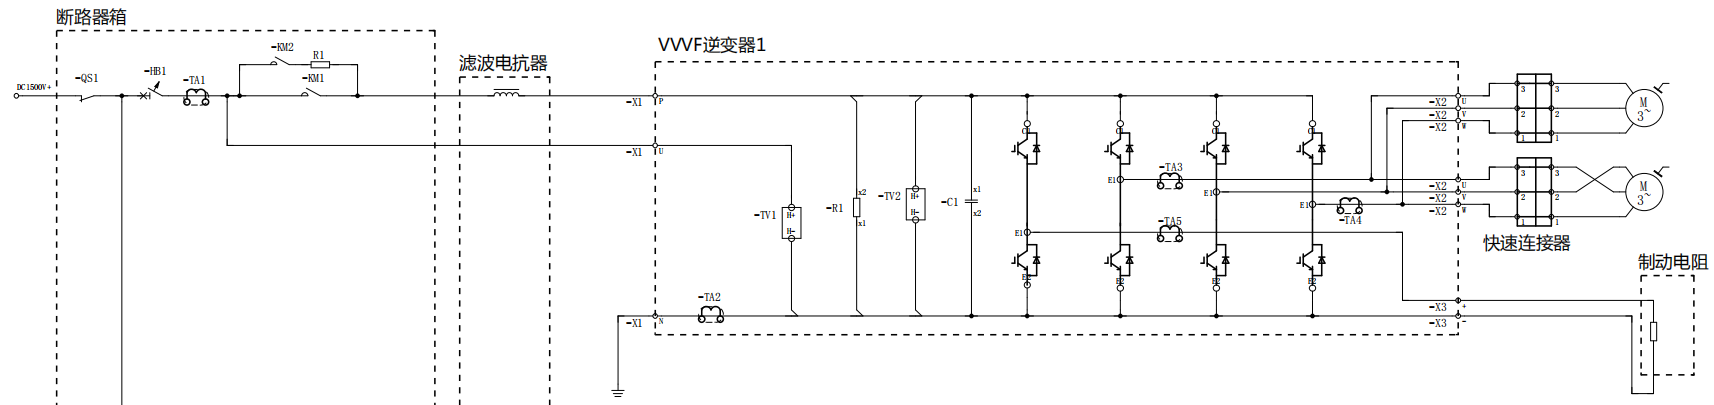
\includegraphics[width=\linewidth]{牵引主电路图.png}
  \caption{牵引主电路图}
  \label{fig:qianyin}
\end{figure}
!!! 参考数据说明文档

% % !TeX root = ../thuthesis-example.tex

\begin{survey}
\label{cha:survey}

\title{Title of the Survey}
\maketitle


\tableofcontents


本科生的外文资料调研阅读报告。


\section{Figures and Tables}

\subsection{Figures}

An example figure in appendix (Figure~\ref{fig:appendix-survey-figure}).

\begin{figure}
  \centering
  
\includegraphics[width=0.6\linewidth]{example-image-a.pdf}
  \caption{Example figure in appendix}
  \label{fig:appendix-survey-figure}
\end{figure}


\subsection{Tables}

An example table in appendix (Table~\ref{tab:appendix-survey-table}).

\begin{table}
  \centering
  \caption{Example table in appendix}
  \begin{tabular}{ll}
    \toprule
    File name       & Description                                         \\
    \midrule
    thuthesis.dtx   & The source file including documentaion and comments \\
    thuthesis.cls   & The template file                                   \\
    thuthesis-*.bst & BibTeX styles                                       \\
    thuthesis-*.bbx & BibLaTeX styles for bibliographies                  \\
    thuthesis-*.cbx & BibLaTeX styles for citations                       \\
    \bottomrule
  \end{tabular}
  \label{tab:appendix-survey-table}
\end{table}


\section{Equations}

An example equation in appendix (Equation~\eqref{eq:appendix-survey-equation}).
\begin{equation}
  \frac{1}{2 \symup{\pi} \symup{i}} \int_\gamma f = \sum_{k=1}^m n(\gamma; a_k) \mathscr{R}(f; a_k)
  \label{eq:appendix-survey-equation}
\end{equation}


\section{Citations}

Example citations in appendix.
\cite{abrahams99tex}
\cite{salomon1995advanced}
\cite{abrahams99tex,salomon1995advanced}


\bibliographystyle{unsrtnat}
\bibliography{ref/appendix}

\end{survey}
       % 本科生:外文资料的调研阅读报告
% % !TeX root = ../thuthesis-example.tex

\begin{translation}
\label{cha:translation}

\title{书面翻译题目}
\maketitle

\tableofcontents


本科生的外文资料书面翻译。


\section{图表示例}

\subsection{图}

附录中的图片示例(图~\ref{fig:appendix-translation-figure})。

\begin{figure}
  \centering
  
\includegraphics[width=0.6\linewidth]{example-image-a.pdf}
  \caption{附录中的图片示例}
  \label{fig:appendix-translation-figure}
\end{figure}


\subsection{表格}

附录中的表格示例(表~\ref{tab:appendix-translation-table})。

\begin{table}
  \centering
  \caption{附录中的表格示例}
  \begin{tabular}{ll}
    \toprule
    文件名          & 描述                         \\
    \midrule
    thuthesis.dtx   & 模板的源文件,包括文档和注释 \\
    thuthesis.cls   & 模板文件                     \\
    thuthesis-*.bst & BibTeX 参考文献表样式文件    \\
    thuthesis-*.bbx & BibLaTeX 参考文献表样式文件  \\
    thuthesis-*.cbx & BibLaTeX 引用样式文件        \\
    \bottomrule
  \end{tabular}
  \label{tab:appendix-translation-table}
\end{table}


\section{数学公式}

附录中的数学公式示例(公式~\eqref{eq:appendix-translation-equation})。
\begin{equation}
  \frac{1}{2 \symup{\pi} \symup{i}} \int_\gamma f = \sum_{k=1}^m n(\gamma; a_k) \mathscr{R}(f; a_k)
  \label{eq:appendix-translation-equation}
\end{equation}


\section{文献引用}

文献引用示例\cite{abrahams99tex}。


% 书面翻译的参考文献
\bibliographystyle{unsrtnat}
\bibliography{ref/appendix}

% 书面翻译对应的原文索引
\begin{translation-index}
  \nocite{salomon1995advanced}
  \bibliographystyle{unsrtnat}
  \bibliography{ref/appendix}
\end{translation-index}

\end{translation}
  % 本科生:外文资料的书面翻译

% 致谢
% !TeX root = ../thuthesis-example.tex

\begin{acknowledgements}
  衷心感谢导师×××教授和物理系××副教授对本人的精心指导。他们的言传身教将使我终生受益。

  在美国麻省理工学院化学系进行九个月的合作研究期间,承蒙 Robert Field 教授热心指导与帮助,不胜感激。

  感谢×××××实验室主任×××教授,以及实验室全体老师和同窗们学的热情帮助和支持!

  本课题承蒙国家自然科学基金资助,特此致谢。
\end{acknowledgements}


% 声明
\statement
% 生成的声明页是否要插入页眉和页脚(默认 empty)
% 仅在需要进行电子签名时,才需要打开这一选项
% 插入的扫描声明页总是会生成页眉(研究生)和页脚,不受这一选项影响
% \statement[page-style=plain]
% 将签字扫描后的声明文件 scan-statement.pdf 替换原始页面
% \statement[file=scan-statement.pdf]

% 个人简历、在学期间完成的相关学术成果
% !TeX root = ../thuthesis-example.tex

\begin{resume}

  \section*{个人简历}

  1997 年 7 月 3 日出生于湖南常德市澧县。

  2014 年 9 月考入清华大学自动化系自动化专业,2018 年 7 月本科毕业并获得理学学士学位。

  2018 年 9 月免试进入清华大学软件工程系攻读软件工程硕士至今。


  \section*{在学期间完成的相关学术成果}

  \subsection*{专利}

  \begin{achievements}
    \item 
  \end{achievements}

\end{resume}


% 指导教师/指导小组学术评语
% !TeX root = ../thuthesis-example.tex

\chapter{指导教师学术评语}

论文提出了……

% 答辩委员会决议书
% !TeX root = ../thuthesis-example.tex

\chapter{答辩委员会决议书}

论文提出了……

论文取得的主要创新性成果包括:

1. ……

2. ……

3. ……

论文工作表明作者在×××××具有×××××知识,具有××××能力,论文××××,答辩××××。

答辩委员会表决,(×票/一致)同意通过论文答辩,并建议授予×××(姓名)×××(门类)学博士/硕士学位。


% 本科生的综合论文训练记录表(扫描版)
% \record{file=scan-record.pdf}

\end{document}
